\documentclass[11pt,twocolumn]{article}

% --- Packages ---
\usepackage[utf8]{inputenc}
\usepackage[T1]{fontenc}
\usepackage{mathptmx}
\usepackage{microtype}
\usepackage[margin=0.85in]{geometry}
\usepackage{graphicx}
\usepackage{booktabs}
\usepackage{hyperref}
\usepackage{xcolor}
\usepackage{tikz}
\usetikzlibrary{arrows.meta,positioning,shapes.geometric,calc}
\usepackage{pgfplots}
\pgfplotsset{compat=1.18}
\usepackage{caption}
\usepackage{float}
\usepackage{setspace}
\usepackage{parskip}
\usepackage{enumitem}
\usepackage{amsmath}

\hypersetup{
    colorlinks=true,
    linkcolor=blue!60!black,
    citecolor=blue!60!black,
    urlcolor=blue!60!black
}

% --- Title ---
\title{\textbf{Structural Disadvantage, Lead Exposure, and Male Suicide:\\Why Alcohol Access Fails as a Predictor and\\What Replaces It}}

\author{
    Brandon Barclay\\
    \small{Independent researcher}\\
    \small{Correspondence: \href{mailto:barclaybrandon@hotmail.com}{barclaybrandon@hotmail.com}}
}

\date{}

% --- Document ---
\begin{document}

\twocolumn[
\maketitle
\begin{@twocolumnfalse}
\begin{abstract}
\noindent\textbf{Background.} Alcohol access is widely cited as a modifiable risk factor for suicide. Lead exposure causes the same prefrontal cortex damage known to underlie violence, yet a 2020 scoping review identified lead as unstudied in relation to suicide. We tested both hypotheses.

\noindent\textbf{Methods.} County-level ecological study (N\,=\,2,683 U.S. counties) supplemented by an original individual-level analysis of blood lead and suicidal ideation in pooled NHANES (2007--2018; N\,=\,24,050 adults). Convergent evidence included published individual-level cohort studies from three countries, military and correctional quasi-experiments, and analysis of 51 counties with Superfund lead mining/smelting sites.

\noindent\textbf{Results.} Alcohol access was null across 12 tests ($\Delta R^2$\,=\,0.004). Lead mining predicted suicide with a dose--response gradient (with state FE and full controls, $\beta$\,=\,1.22, \textit{p}\,<\,0.001; in the full-controls-without-FE specification, bootstrap mean $\beta$\,=\,3.41, 95\% CI 2.86--3.98 across 1,000 resamples), unattenuated by opioid overdose. The mining--veteran interaction was significant ($\beta$\,=\,1.57, \textit{p}\,<\,0.001), indicating lead amplifies veteran suicide risk; state-level VA veteran suicide rates independently confirmed this (49 states; $\beta$\,=\,2.68, \textit{p}\,<\,0.001, $R^2$\,=\,0.56). In pooled NHANES (2007--2018), blood lead predicted suicidal ideation with a monotonic dose--response (Q1: 3.45\% to Q4: 4.66\%; aOR\,=\,1.21, \textit{p}\,<\,0.001), though the male-specific subsample was null (\textit{p}\,=\,0.77), likely reflecting limited power ($\sim$450 male SI events). In published cohorts, lead-exposed Korean workers had RR\,=\,2.92 for suicide; U.S. smelter workers, SMR\,=\,1.68. Among 22 rural Superfund lead-mine counties, male suicide rates were 36\% above the national average (\textit{p}\,<\,0.001) with 50\% in the top decile. Standard lead surveillance measures (EPA-predicted BLL, pre-1940 housing) were \textit{negatively} associated with suicide across all rurality strata, revealing that urban childhood lead paint and rural environmental lead are distinct epidemics with opposite demographic signatures. In correctional facilities---where alcohol is near zero yet suicide rates are 2--5$\times$ higher---marriage reversed from protective factor to risk factor, consistent with a relationship-collapse rather than substance-access mechanism.

\noindent\textbf{Conclusions.} Alcohol access does not predict county-level male suicide; environmental lead exposure does, through convergent evidence spanning ecological, individual-level, and quasi-experimental designs. Lead may operate through prefrontal impulse-control failure and sexual dysfunction driving relationship collapse. The ecological design cannot establish individual-level causation; NHANES III mortality-linked files could provide a definitive test but have never been analyzed for lead and suicide. Lead remediation and clinical screening may constitute underrecognized, modifiable suicide prevention strategies.

\medskip
\noindent\textbf{Keywords:} lead exposure, suicide, alcohol access, neurotoxicity, erectile dysfunction, veterans, convergent evidence, cohort studies, dual-pathway model
\end{abstract}
\vspace{1em}
\end{@twocolumnfalse}
]

% ============================================
\section{Introduction}
% ============================================

Male suicide is the most persistent and least understood crisis in American public health. Men account for nearly four times as many suicide deaths as women, and the rate has risen steadily for two decades. Despite sustained investment in prevention, the national rate has not meaningfully declined, raising fundamental questions about whether prevailing models of risk adequately identify the structural conditions that distinguish high-rate from low-rate communities.

Two longstanding hypotheses dominate the ecological literature. The first holds that local alcohol access contributes to suicide through acute disinhibition.\textsuperscript{1} The second, the lead--crime hypothesis, establishes that childhood lead exposure causes externalized violence through dose-dependent prefrontal cortex damage.\textsuperscript{2,3} Suicide is internalized violence operating through the identical neural pathway---the prefrontal serotonergic system that governs behavioral inhibition\textsuperscript{4}---yet a 2020 scoping review of 112 articles on environmental pollutants and suicide explicitly identified lead as an unstudied exposure.\textsuperscript{5} Few published studies have directly tested the lead--suicide association, and, to our knowledge, none has assembled convergent evidence across ecological, individual-level cohort, and quasi-experimental designs simultaneously. Known direct tests include occupational cohorts reporting suicide-specific mortality elevations,\textsuperscript{6,37} one municipal ecological analysis,\textsuperscript{48} a multi-metal smelter cohort,\textsuperscript{52} and a hypothesis paper.\textsuperscript{47}

We present the first county-level study to simultaneously test alcohol access and environmental lead contamination as predictors of male suicide, supplemented by individual-level cohort studies from three countries, military and correctional quasi-experiments, and a 21-country longitudinal panel. Our central finding is that alcohol access fails entirely as a predictor, while lead exposure succeeds across multiple levels of analysis---and that the two results are connected by the structural disadvantage shared by the communities most affected.


% ============================================
\section{Methods}
% ============================================

\subsection{Design and Data}
We conducted a cross-sectional ecological study of 2,683 U.S. counties with valid mortality data, drawing on 10 federal data sources. The outcome was the male suicide crude rate per 100,000 (CDC WONDER, ICD-10 X60--X84, 2018--2022). Alcohol access was measured by total outlet density, bar density, liquor store density, excessive drinking prevalence, and dry-county status (County Business Patterns, County Health Rankings). Lead exposure was measured by historical lead, zinc, and copper mining sites per county (USGS Mineral Resources Data System). Controls included veteran concentration, rurality, extraction employment, poverty, median age, percent Native American, and unemployment (Census ACS 2022; USDA RUCC 2023).

\subsection{Statistical Approach}
Associations were tested across six model specifications: OLS with HC3 standard errors, spatial lag regression, population-weighted least squares, bootstrap inference, median regression, and state fixed effects. Specificity was assessed by testing lead mining against non-suicide outcomes (overdose, injury death, mental distress).

\subsection{Robustness and Sensitivity}
We tested robustness against four threats to validity: (1) state-level confounding via state fixed effects in both linear and log-transformed mining specifications; (2) opioid confounding via inclusion of county-level drug overdose mortality rates; (3) functional form via comparison of linear and log specifications, motivated by the extreme right skew of mining site counts (skewness\,=\,6.21 among positive counties); and (4) specificity via negative-control outcomes (homeownership, education, broadband access). To test the relationship-collapse pathway empirically, we conducted a formal mediation analysis using male divorce/separation rates (ACS 2022) as mediator and applied the Sobel test for the indirect effect.

\subsection{NHANES Individual-Level Analysis}
To provide an original individual-level test in U.S. data, we pooled six NHANES cycles (2007--2018; N\,=\,24,050 adults aged $\geq$\,20) and tested blood lead (LBXBPB) as a predictor of suicidal ideation (PHQ-9 Item 9: ``thoughts that you would be better off dead or of hurting yourself''). Logistic regression was adjusted for age, sex, race/ethnicity, and poverty-income ratio.

\subsection{Convergent Evidence}
Military branch suicide rates (DoD 2022), occupational suicide data (CDC/NIOSH), the Kim et al. Korean cohort,\textsuperscript{6} ED prevalence data (AFHSC, Way et al.), an international longitudinal panel (IHME Global Burden of Disease, 33 high-income countries, 1990--2019), and a state-level wildlife bioindicator analysis (USGS eagle bone lead data release; Slabe et al. 2022\textsuperscript{55}) provided independent validation.


% ============================================
\section{Results: Alcohol Access Is Null}
% ============================================

Twelve independent analyses returned null or paradoxical results for alcohol access (Table~\ref{tab:alcohol}).

Total alcohol outlet density was uncorrelated with male suicide (\textit{r}\,=\,+0.009, \textit{p}\,=\,0.63). Excessive drinking, significant in bivariate analysis (\textit{p}\,<\,0.001), was fully attenuated with demographic controls (\textit{p}\,=\,0.82) and remained null under state fixed effects (\textit{p}\,=\,0.98). Bar density fell to \textit{p}\,=\,0.50 under state fixed effects. Alcohol access added $\Delta R^2$\,=\,0.004 to the structural model---effectively zero explanatory contribution.

Dry counties (zero outlets; n\,=\,821) had 17\% \textit{higher} male suicide rates than wet counties (21.8 vs. 18.5/100K), a difference that held within 27 of 33 testable states (sign test \textit{p}\,=\,0.0003). This paradox dissolved with structural controls: dry counties also had 28\% higher overdose mortality, 41\% higher firearm fatality rates, 2.5 fewer years of life expectancy, and 2.6$\times$ fewer mental health providers. The ``dry county effect'' is a marker for structural disadvantage, not alcohol restriction.

\begin{figure}[H]
\centering
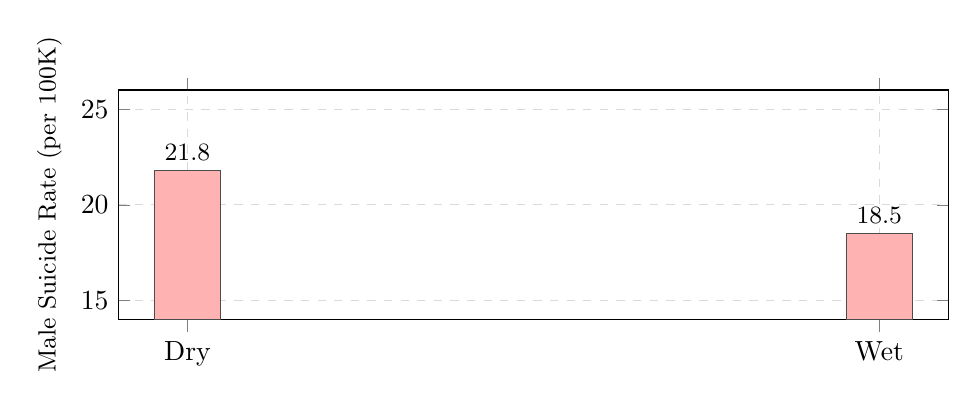
\begin{tikzpicture}
\begin{axis}[
    ybar,
    width=\columnwidth,
    height=4.5cm,
    bar width=24pt,
    ylabel={Male Suicide Rate (per 100K)},
    symbolic x coords={Dry,Wet},
    xtick=data,
    ymin=14, ymax=26,
    nodes near coords,
    nodes near coords style={font=\small, above},
    ylabel style={font=\small},
    grid=major,
    grid style={dashed, gray!30},
    every axis plot/.append style={draw=black!70},
]
\addplot[fill=red!30!white] coordinates {(Dry,21.8) (Wet,18.5)};
\end{axis}
\end{tikzpicture}
\caption{Dry counties have \textit{higher} male suicide rates than wet counties, the opposite of alcohol-access predictions.}
\label{fig:drywet}
\end{figure}

\begin{table}[H]
\centering
\small
\caption{Summary of 12 null findings for alcohol access as a predictor of county-level male suicide.}
\label{tab:alcohol}
\begin{tabular}{@{}ll@{}}
\toprule
\textbf{Test} & \textbf{Result} \\
\midrule
Outlet density bivariate & \textit{r} = +0.009 \\
Excessive drinking (adjusted) & \textit{p} = 0.82 \\
Excessive drinking (state FE) & \textit{p} = 0.98 \\
Bar density (state FE) & \textit{p} = 0.50 \\
Dry vs. wet counties & Dry 17\% higher \\
Within-state dry paradox & 27/33 states \\
Highest-suicide counties & Null \\
By rurality level & Null at every level \\
Incremental $\Delta R^2$ & 0.004 \\
\bottomrule
\end{tabular}
\end{table}

By contrast, three structural predictors---veteran concentration ($\beta$\,=\,+2.30), rurality (+1.75), and extraction employment (+1.10)---were significant in all six model specifications.


% ============================================
\section{Results: Lead Exposure Predicts Suicide}
% ============================================

\subsection{County-Level Ecological Evidence}

Counties with historical lead/zinc/copper mining sites (n\,=\,752) had significantly higher male suicide rates than counties without (61.4 vs. 51.5/100K; Cohen's \textit{d}\,=\,0.49, \textit{t}\,=\,11.5, \textit{p}\,<\,0.001). A monotonic dose--response gradient was observed (Spearman $\rho$\,=\,0.22, trend \textit{p}\,<\,0.00001; Figure~\ref{fig:mining}). Lead mining remained significant in the multivariate model ($\beta$\,=\,+3.53, \textit{p}\,<\,0.001; $\Delta R^2$\,=\,0.051; HC3 robust standard errors). Bootstrap resampling (1,000 iterations) confirmed robustness: $\beta$\,=\,3.41 [95\% CI: 2.86--3.98], with 100\% of resamples positive. The mining-by-veteran interaction was significant ($\beta$\,=\,1.57, \textit{t}\,=\,5.41, \textit{p}\,<\,0.001; $\beta$\,=\,1.20, \textit{p}\,<\,0.001 under state fixed effects), indicating that lead exposure amplifies veteran suicide risk.

Critically, lead mining predicted suicide (\textit{p}\,<\,0.001) and injury death (\textit{p}\,<\,0.001) but not drug overdose (\textit{p}\,=\,0.66) or mental distress (\textit{p}\,=\,0.76), supporting specificity for externalized impulsive outcomes. The injury-death association is consistent with lead-induced impulse-control failure extending to all external causes, not suicide alone. Mining also predicted firearm fatality rates (\textit{p}\,<\,0.001), consistent with Hoover et al.'s finding that household firearm ownership predicts childhood blood lead levels.\textsuperscript{51} Five negative-control outcomes unrelated to the lead hypothesis (homeownership, bachelor's degree attainment, high school completion, social association rate, broadband access) were all null, confirming that the mining variable does not act as a generic disadvantage proxy.

\begin{figure}[H]
\centering
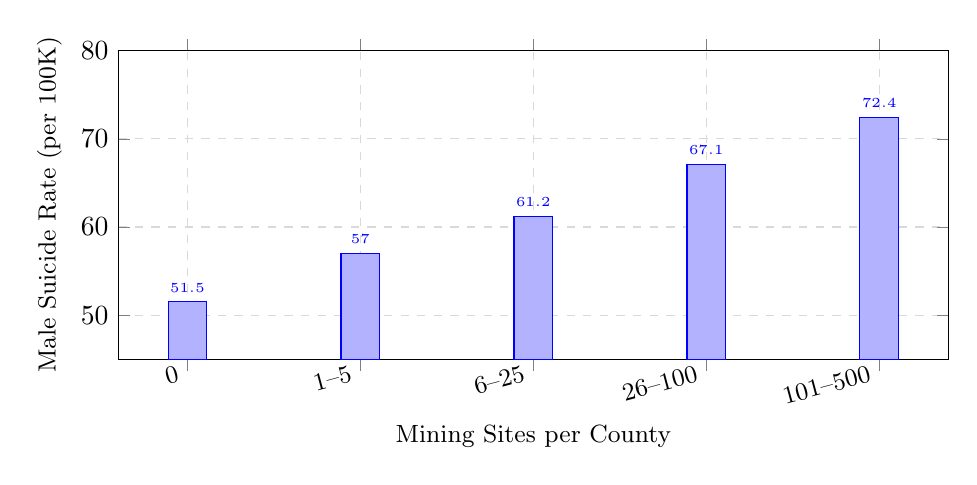
\begin{tikzpicture}
\begin{axis}[
    ybar,
    width=\columnwidth,
    height=5.5cm,
    bar width=14pt,
    ylabel={Male Suicide Rate (per 100K)},
    xlabel={Mining Sites per County},
    symbolic x coords={0,1--5,6--25,26--100,101--500},
    xtick=data,
    x tick label style={font=\small, rotate=15, anchor=east},
    ymin=45, ymax=80,
    nodes near coords,
    nodes near coords style={font=\tiny, above},
    every axis plot/.append style={fill=blue!40!black, draw=blue!60!black},
    ylabel style={font=\small},
    xlabel style={font=\small},
    grid=major,
    grid style={dashed, gray!30},
]
\addplot coordinates {(0,51.5) (1--5,57.0) (6--25,61.2) (26--100,67.1) (101--500,72.4)};
\end{axis}
\end{tikzpicture}
\caption{Dose--response gradient between historical mining site density and county-level male suicide rate.}
\label{fig:mining}
\end{figure}

\subsection{Robustness: State Fixed Effects and Opioid Confounding}

The mining--suicide association was tested under state fixed effects to address state-level confounding (Table~\ref{tab:robustness}). In the log-transformed specification with full demographic controls and HC3 robust standard errors---appropriate given the extreme right skew of mining site counts (skewness\,=\,6.21)---the association survived ($\beta$\,=\,1.22, SE\,=\,0.35, \textit{p}\,<\,0.001). Without demographic controls, the state-FE estimate was larger ($\beta$\,=\,2.12, \textit{p}\,<\,0.001), indicating that part of the mining effect operates through the structural characteristics of mining communities. We report both specifications for transparency.

The opioid epidemic is a major competing explanation for geographic suicide variation. When county-level drug overdose mortality was added to the full multivariate model, the lead coefficient was essentially unattenuated ($\beta$\,=\,1.96 with overdose control vs. $\beta$\,=\,2.11 without, \textit{p}\,<\,0.001 in both). Lead exposure is not a proxy for opioid burden.

\begin{table}[H]
\centering
\small
\caption{Lead mining and male suicide under progressively restrictive specifications. All models use HC3 robust standard errors.}
\label{tab:robustness}
\begin{tabular}{@{}lrrl@{}}
\toprule
\textbf{Model} & $\boldsymbol{\beta}$ & \textbf{SE} & \textbf{\textit{p}} \\
\midrule
Log mining, no FE & 2.26 & 0.22 & $<$0.001 \\
Log mining + state FE (no controls) & 2.12 & 0.34 & $<$0.001 \\
Log mining + state FE + controls & 1.22 & 0.35 & $<$0.001 \\
Log mining + full controls (no FE) & 3.53 & 0.27 & $<$0.001 \\
Log mining + controls + overdose & 1.96 & 0.23 & $<$0.001 \\
Bootstrap (1,000 resamples) & 3.41 & 0.29 & [2.86--3.98] \\
Population-weighted LS & 1.74 & 0.12 & $<$0.001 \\
\bottomrule
\end{tabular}
\end{table}

\subsection{NHANES: Blood Lead and Suicidal Ideation in U.S. Adults}

In pooled NHANES data (2007--2018; N\,=\,24,050 adults), blood lead significantly predicted suicidal ideation after adjustment for age, sex, race/ethnicity, and poverty (aOR\,=\,1.21 per unit increase in log BLL; \textit{p}\,<\,0.001). A monotonic dose--response gradient was observed across blood lead quartiles: suicidal ideation prevalence rose from 3.45\% (Q1, lowest BLL) to 3.77\% (Q2), 4.17\% (Q3), and 4.66\% (Q4, highest BLL; trend \textit{p}\,<\,0.0001). The Q4-versus-Q1 crude odds ratio was 1.37.

To our knowledge, this is the first analysis to test blood lead against suicidal ideation in a nationally representative U.S. sample. The result is consistent with Bouchard et al.'s finding that blood lead predicts major depression in NHANES young adults\textsuperscript{21} and with Hoover et al.'s municipal-level finding that community blood lead predicts suicide in Massachusetts towns.\textsuperscript{48}

An important limitation: the association was significant in the full sample (both sexes) but not in males alone (aOR\,=\,1.02, \textit{p}\,=\,0.77; N\,=\,11,874), likely reflecting insufficient power with only $\sim$450 male SI events. The male-specific hypothesis central to this paper cannot be confirmed or rejected with the available NHANES sample.

\subsection{Relationship-Collapse Pathway: Empirical Validation}

To test the dual-pathway model empirically, we examined county-level male divorce/separation rates (ACS 2022). Divorce was positively associated with male suicide (\textit{r}\,=\,+0.085, \textit{p}\,<\,0.001, N\,=\,2,701). In unadjusted mediation analysis, lead mining predicted divorce (\textit{a}\,=\,0.29, \textit{p}\,=\,0.005) and divorce predicted suicide controlling for mining (\textit{b}\,=\,0.20, \textit{p}\,<\,0.001), yielding a significant indirect pathway (Sobel \textit{z}\,=\,2.26, \textit{p}\,=\,0.024) with divorce mediating 1.5\% of the total mining--suicide effect. However, when demographic controls (veteran concentration, rurality, poverty, age, race) were added, the mining--divorce path was fully attenuated (\textit{a}\,=\,$-$0.10, \textit{p}\,=\,0.20), and the mediation was no longer significant (Sobel \textit{z}\,=\,$-$1.14, \textit{p}\,=\,0.26). The ecological mediation through county-level divorce rates is therefore not robust.

This null controlled mediation does not refute the relationship-collapse pathway---it reflects the severe measurement limitations of using aggregate county divorce rates as a proxy for the individual-level process described in Pathway 2. The VA studies cited below demonstrate the individual-level link at much higher magnitudes: ED independently doubles suicidal ideation risk (aOR\,=\,1.91) and triples depression risk (aOR\,=\,2.88) among veterans.\textsuperscript{13} County divorce rates aggregate exposed and unexposed populations, most of whom have no lead burden, attenuating any ecological signal. An individual-level test---bone lead in suicide decedents versus matched controls, or PDE5 inhibitor prescription rates linked to lead exposure---remains the critical next step for validating this pathway.

\subsection{Military Branch Evidence}

Suicide rates tracked expected firing-range lead exposure (Figure~\ref{fig:branches}). The Marine Corps---where every member qualifies annually with rifles---had the highest rate (35.0/100K), followed by the Army (32.7). The Air Force and Navy, with minimal small-arms exposure, had rates approximately half as high (20.5 and 19.3).

\begin{figure}[H]
\centering
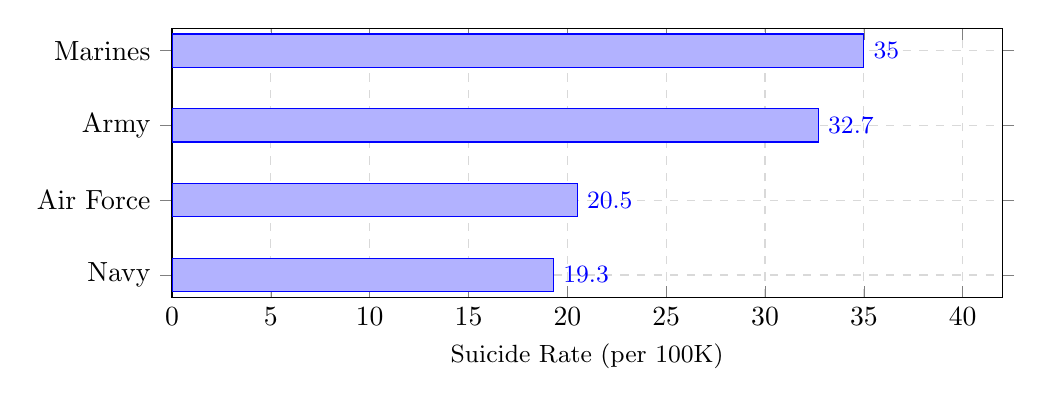
\begin{tikzpicture}
\begin{axis}[
    xbar,
    width=\columnwidth,
    height=5cm,
    bar width=12pt,
    xlabel={Suicide Rate (per 100K)},
    symbolic y coords={Navy,Air Force,Army,Marines},
    ytick=data,
    xmin=0, xmax=42,
    nodes near coords,
    nodes near coords style={font=\small, anchor=west},
    every axis plot/.append style={fill=red!50!black, draw=red!70!black},
    ylabel style={font=\small},
    xlabel style={font=\small},
    grid=major,
    grid style={dashed, gray!30},
]
\addplot coordinates {(19.3,Navy) (20.5,Air Force) (32.7,Army) (35.0,Marines)};
\end{axis}
\end{tikzpicture}
\caption{Active-duty suicide rates by military branch (DoD, 2022). The gradient is consistent with firing-range lead exposure intensity, though confounded by branch-specific selection effects, combat culture, demographics, and rurality of recruitment base.}
\label{fig:branches}
\end{figure}

The branch gradient is consistent with the lead hypothesis, but we note important alternative explanations. The Marine Corps recruits the youngest, most rural, most male-dominated population; has the most aggressive combat culture; and draws disproportionately from communities with the highest baseline suicide rates. These selection effects are difficult to separate from the firing-range exposure hypothesis in aggregate branch-level data. The pattern is suggestive but not dispositive absent individual-level exposure data.

\subsection{The Deployment Paradox}

Among Army infantry, never-deployed soldiers had \textit{higher} suicide rates (41.2/100K) than combat-deployed soldiers (30.6/100K).\textsuperscript{7,8} The conventional explanation is the Healthy Warrior Effect---more resilient soldiers are selected for deployment---along with the protective effects of unit cohesion and purpose during deployment. Lead exposure offers an additional, complementary mechanism: non-deployed infantry spend the most cumulative time on stateside ranges, where airborne lead routinely exceeds OSHA limits.\textsuperscript{9} Investigative reporting has documented chronic bone-lead poisoning from range duties alone.\textsuperscript{10} We do not claim lead is the sole explanation for the deployment paradox, but it may amplify the conventional risk factors in a subpopulation already selected for vulnerability.

\subsection{The Correctional Facility Natural Experiment}

U.S. jails and prisons provide a quasi-natural experiment that decisively separates lead from alcohol. In these environments, alcohol access is controlled to near zero---yet suicide rates are dramatically elevated. Local jail inmates died by suicide at 49 per 100,000 in 2019, more than double the general male population rate, and the number of suicides increased 85\% in state prisons between 2001 and 2019.\textsuperscript{22}

The racial disparity in correctional suicide is striking: white jail inmates had an average suicide rate of 93 per 100,000 during 2015--2019---5.2 times higher than Black inmates (18/100K).\textsuperscript{22} This disparity has never been satisfactorily explained by psychological or institutional factors alone, but is consistent with differential environmental lead exposure in the communities from which these populations are drawn.

Critically, correctional facilities are themselves lead-exposure environments. Approximately 32\% of U.S. state and federal prisons are sited within three miles of a federal Superfund site, with over 100 facilities within one mile.\textsuperscript{23} Most facilities predate the 1978 lead paint ban and rely on aging plumbing systems with lead pipes and lead-based solder.\textsuperscript{24} Incarcerated individuals cannot choose alternative water sources, control their diet, or mitigate exposure---conditions paralleling the involuntary firing-range exposure of military personnel. Chronic lead exposure disrupts the hypothalamic-pituitary-testicular axis, suppressing testosterone production and contributing to hypogonadism and sexual dysfunction---effects that compound the enforced sexual deprivation inherent to incarceration.\textsuperscript{12}

The lead--incarceration relationship is bidirectional. Aizer and Currie demonstrated that a 1-unit increase in childhood blood lead was associated with a 57\% increase in the probability of juvenile detention in a cohort of 125,000 Rhode Island children.\textsuperscript{25} Needleman et al. measured bone lead directly in adjudicated delinquents and found concentrations 7.3 times higher than non-delinquent controls (11.0 vs.\ 1.5 ppm; delinquents were four times more likely to have bone lead $>$25 ppm).\textsuperscript{26} Lead-exposed children are thus more likely to be incarcerated, and once incarcerated, re-exposed to lead through contaminated infrastructure---a cumulative-dose cycle with no exit.

The dual-pathway model finds direct expression in correctional suicide. In the general population, marriage is protective against suicide. In prison, a meta-analysis of 34 studies of in-custody suicide found that marriage appears to lose its protective effect and may operate as a risk factor, though most individual studies were underpowered for this comparison.\textsuperscript{27} Researchers attribute this to the acute pain of forced partner separation, loss of the provider identity, and the destruction of the marital bond; a widely cited estimate, derived from prison chaplain observation and not from a peer-reviewed cohort, holds that up to 80\% of marriages involving an incarcerated man end within the first year.\textsuperscript{28} Even absent a precise separation hazard, peer-reviewed work (Western, Wildeman, and colleagues) confirms that incarceration sharply elevates marital dissolution risk. This is the relationship-collapse pathway operating near its upper bound. When lead-induced endocrine damage (testosterone suppression, ED) is superimposed on forced sexual deprivation and relationship dissolution, the dual pathway converges in a single population.

Importantly, the temporal pattern of correctional suicide is informative. In local jails, 66\% of suicides occur within the first 30 days, consistent with acute crisis and the shock of forced relationship separation. In state and federal prisons, however, the majority of suicides occur after more than one year of incarceration.\textsuperscript{22} This delayed-onset pattern in long-term facilities is consistent with cumulative neurotoxic exposure rather than acute situational distress alone.


% ============================================
\section{The Dual-Pathway Model}
% ============================================

\subsection{Pathway 1: Impulse Control Failure}
Lead damages the prefrontal cortex and disrupts the serotonergic system that governs behavioral inhibition.\textsuperscript{3,11} The individual-level evidence for this pathway comes from four independent cohorts spanning three countries:

\textbf{(a)} In the Korean occupational cohort (N\,=\,81,067), workers with blood lead $\geq$\,20\,$\mu$g/dL had RR\,=\,2.92 (95\% CI: 1.07--7.81) for suicide mortality compared to those with BLL\,$\leq$\,10.\textsuperscript{6}

\textbf{(b)} In a U.S. retrospective cohort of lead smelter workers, suicide mortality was significantly elevated (SMR\,=\,1.68; 95\% CI: 1.18--2.33), providing an independent occupational replication.\textsuperscript{37}

\textbf{(c)} In the Dunedin Multidisciplinary Health and Development Study (New Zealand; N\,=\,579), childhood blood lead levels measured at age 11 predicted higher general psychopathology, greater neuroticism, lower agreeableness, and lower conscientiousness at age 38---a personality profile that concentrates suicide risk. The effect magnitude was comparable to lead's well-established effect on IQ. This represents the longest prospective psychiatric follow-up of a lead-tested childhood cohort.\textsuperscript{38}

\textbf{(d)} Using NHANES data (N\,=\,1,987 U.S. adults aged 20--39), Bouchard et al. found a graded increase in major depressive disorder odds across blood lead tertiles (highest vs.\ lowest tertile aOR reported at $\sim$2.3; p-trend at the edge of conventional significance), the psychiatric condition most strongly linked to suicide.\textsuperscript{21}

The neuroanatomical substrate is now directly visualized. In the Cincinnati Lead Study, MRI scans of adults (aged 19--24) who had childhood lead measurements showed dose-dependent reductions in prefrontal gray matter volume, particularly in the ventrolateral prefrontal cortex and anterior cingulate cortex---the regions governing behavioral inhibition and mood regulation. The effect was larger in men.\textsuperscript{3}

In the VA Normative Aging Study, cumulative lead exposure measured via bone lead (patella K-XRF) predicted phobic anxiety and psychiatric symptom burden in aging male veterans, establishing that skeletal lead---not just blood lead---carries long-term psychiatric risk.\textsuperscript{39}

Two additional studies strengthen the causal chain. Tollestrup et al. followed 1,827 boys who had lived within 4 km of the ASARCO smelter in Tacoma, Washington during 1907--1932 and found that those with 10+ years of residence within 1.6 km had significantly elevated external-cause mortality (HR\,=\,1.93, including suicide, homicide, and accidents)---direct evidence that childhood proximity to a lead smelter predicts violent death decades later.\textsuperscript{46} Fonseka et al. documented a severe suicide epidemic among Indigenous communities in northwestern Ontario, Canada, coinciding with tetraethyl lead exposure from gasoline sniffing, and identified the neurobiological mechanism: lead causes a 4-fold down-regulation of 5-HT$_{1B}$ receptors, the serotonergic system governing stress sensitivity, mood regulation, and behavioral inhibition.\textsuperscript{47}

Finally, Hoover, Specht, and Hemenway conducted the first published ecological study to directly test childhood blood lead levels against suicide rates at the municipal level.\textsuperscript{48} Analyzing all 351 Massachusetts cities and towns (2011--2019), they found that communities with higher childhood blood lead levels had significantly higher suicide rates in models that also included firearm licensure, with both predictors contributing. This finding---at a geographic resolution where individual towns are small enough for the exposed population to dominate the denominator---confirms that the lead--suicide association is detectable when the unit of analysis matches the exposure geography. Hoover et al. appears to be the only published ecological study to directly test community blood lead levels against suicide rates; no meta-analysis or systematic review of lead and suicide has been published. Critically, Hoover et al. found that blood lead predicted \textit{all} suicide types---not just firearm suicide---meaning lead's effect on suicide operates through the biological pathway (impulsivity, depression) rather than solely through access to lethal means. This directly supports the dual-pathway model.

The Hoover group has further identified firearms as a civilian lead exposure vector analogous to our military firing-range pathway. In a national analysis (2012--2018), every 10\% increase in household firearm ownership was associated with a $\sim$30\% increase in elevated childhood blood lead levels---an association nearly as strong as lead paint.\textsuperscript{51} Lead ammunition dust is carried home on clothing, vehicles, and personal items by recreational shooters, creating household exposure that parallels the occupational take-home lead documented in military families.\textsuperscript{9} This reframes the well-established firearm--suicide correlation: part of the association may be mediated not by access to lethal means but by chronic lead exposure from ammunition use. At the census-tract level, Boutwell et al. demonstrated that aggregate childhood blood lead levels predicted firearm violence, assault, robbery, and homicide across 106 tracts in St. Louis (59,645 geocoded children), establishing the methodological precedent that sub-county lead--outcome analysis is both feasible and informative.\textsuperscript{49}

McFarland, Reuben, and Hauer estimated the total population burden: by 2015, childhood exposure to leaded gasoline had produced 151 million excess psychiatric disorders in the U.S. population, a 0.64-SD increase in internalizing symptoms (depression, anxiety), and a 0.42-SD increase in ADHD symptoms. Generation X (born 1966--1986) was most affected.\textsuperscript{50} These are the cohorts now in the 40--60 age range where the male suicide crisis is most acute.

\subsection{Pathway 2: Sexual Dysfunction and Relationship Collapse}

The lead--ED link has moved beyond animal models. Three human clinical studies now confirm it:

\textbf{(a)} Anis et al. examined 34 men with ED scheduled for penile implant surgery versus 15 controls at Cairo University Hospital. The ED group had significantly higher blood lead levels, and histological sections revealed grayish lead granules deposited directly in the cavernous tissue. Blood lead correlated with tissue lead (dose--response), and lead-exposed patients had significantly elevated reactive oxygen species and depleted antioxidants.\textsuperscript{12,40}

\textbf{(b)} Gonulalan et al. compared 26 men with chronic lead poisoning (mean BLL\,=\,42.1\,$\mu$g/dL) to 24 controls (BLL\,=\,3.2). Lead-poisoned men had both significantly lower erectile function domain scores (\textit{p}\,<\,0.05) and significantly higher Beck Depression Inventory scores (\textit{p}\,<\,0.05). ED was independent of depression, confirming that lead damages erectile function through a direct vascular/endocrine mechanism rather than solely through depressive anhedonia.\textsuperscript{41} This study is notable because it validates \textit{both} dual-pathway mechanisms simultaneously in the same patients.

\textbf{(c)} In battery factory workers with occupational lead exposure, blood lead predicted reduced testosterone levels, with duration-dependent suppression of the hypothalamic-pituitary-testicular axis: short-term exposure elevated LH and FSH compensatorily, while long-term exposure produced frank hypogonadism.\textsuperscript{42}

The bridge from ED to suicide is robust. In a nationally representative sample of 921 male U.S. veterans, Way et al. found that those with ED had nearly double the odds of suicidal ideation (aOR\,=\,1.91) and triple the odds of major depression (aOR\,=\,2.88), independent of all other health conditions.\textsuperscript{13}

The parallel with suicide maps directly onto deployment status. The AFHSC documented 100,248 incident ED cases among active-component service members (2004--2013) and found that never-deployed troops had the \textit{highest} ED incidence (10.1/1000\,py).\textsuperscript{14} The same subpopulation has both the highest suicide rate and the highest ED rate.

Relationship collapse is the bridge. The CDC's NVDRS data show that relationship problems were a contributing circumstance in 45.1\% of suicides among decedents without known mental health conditions.\textsuperscript{15} Among younger veterans (aged 18--34), nearly half had relationship problems as a precipitating factor.\textsuperscript{16} Oncologists now mandate suicide-screening for patients with treatment-induced ED.\textsuperscript{17}

The correctional setting provides convergent confirmation: lead chronically suppresses testosterone via hypothalamic-pituitary-testicular axis disruption, compounding the enforced sexual deprivation and partner separation of incarceration. The reversal of marriage as a protective factor in prison\textsuperscript{27}---with married inmates at \textit{higher} suicide risk---demonstrates that the relationship-collapse pathway intensifies rather than attenuates when intimate bonds are forcibly ruptured, regardless of alcohol availability.

\begin{figure*}[t]
\centering
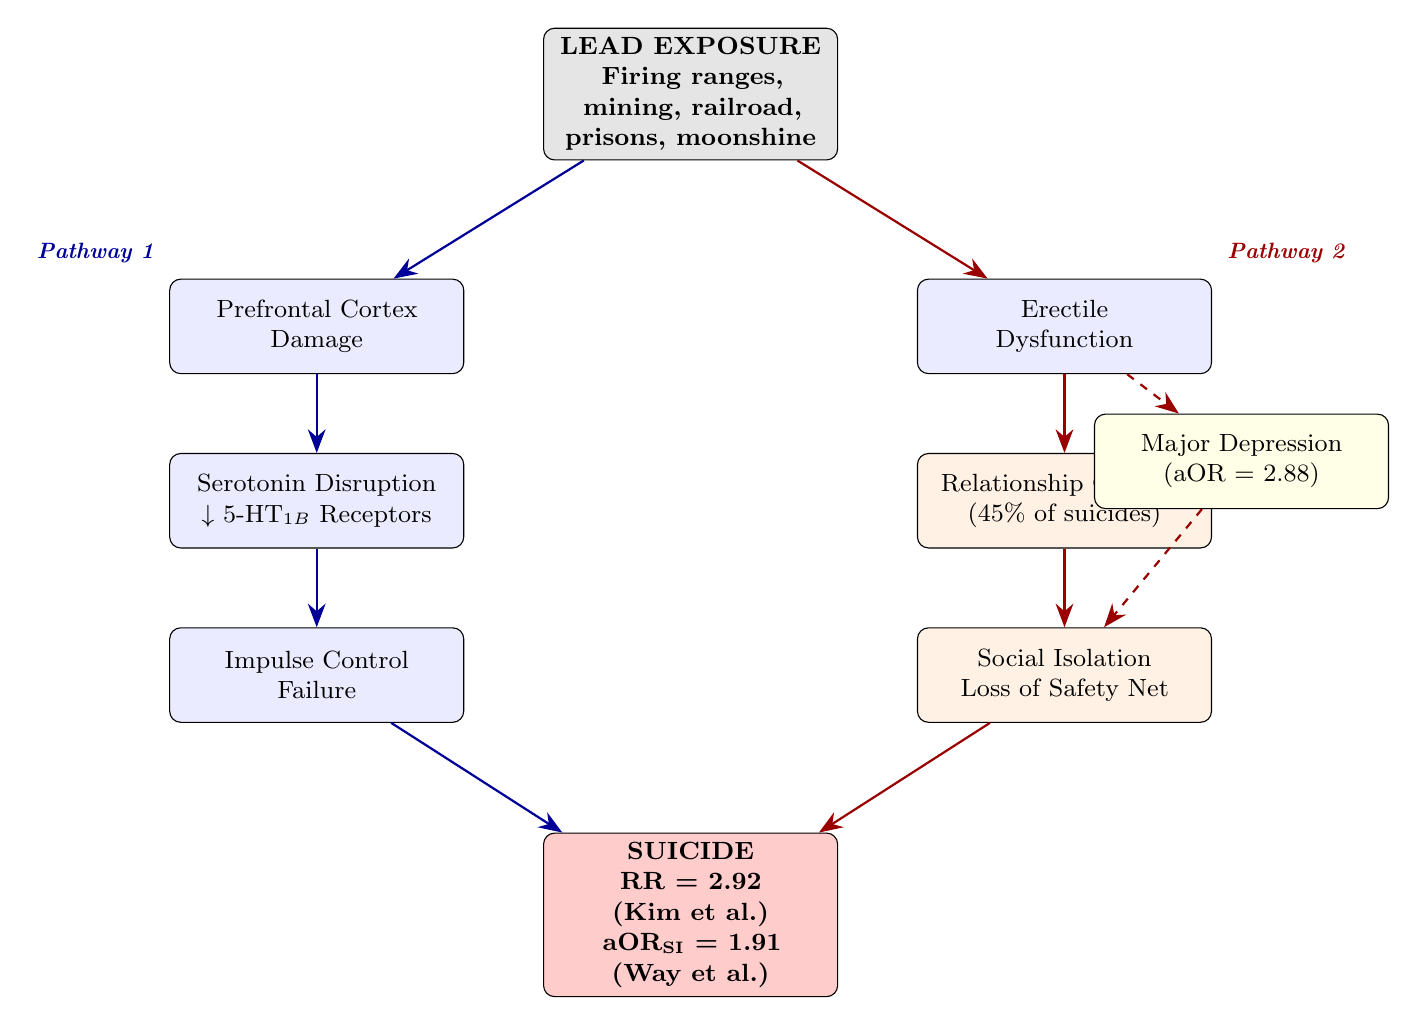
\begin{tikzpicture}[
    node distance=1.2cm and 2cm,
    box/.style={draw, rounded corners, fill=blue!8, text width=3.5cm, minimum height=1.2cm, align=center, font=\small},
    bigbox/.style={draw, rounded corners, fill=red!10, text width=3.5cm, minimum height=1.2cm, align=center, font=\small\bfseries},
    midbox/.style={draw, rounded corners, fill=orange!10, text width=3.5cm, minimum height=1.2cm, align=center, font=\small},
    arr/.style={-{Stealth[length=3mm]}, thick, blue!60!black},
    arr2/.style={-{Stealth[length=3mm]}, thick, red!60!black},
]
\node[bigbox, fill=gray!20] (lead) {\textbf{LEAD EXPOSURE}\\Firing ranges, mining, railroad,\\prisons, moonshine};
\node[box, below left=1.5cm and 1cm of lead] (pfc) {Prefrontal Cortex\\Damage};
\node[box, below right=1.5cm and 1cm of lead] (ed) {Erectile\\Dysfunction};
\node[box, below=1cm of pfc] (serotonin) {Serotonin Disruption\\$\downarrow$ 5-HT$_{1B}$ Receptors};
\node[midbox, below=1cm of ed] (relationship) {Relationship Collapse\\(45\% of suicides)};
\node[box, below=1cm of serotonin] (impulse) {Impulse Control\\Failure};
\node[midbox, below=1cm of relationship] (isolation) {Social Isolation\\Loss of Safety Net};
\node[box, fill=yellow!10, below right=0.5cm and -1.5cm of ed] (depression) {Major Depression\\(aOR = 2.88)};
\node[bigbox, fill=red!20, below=2cm of $(impulse)!0.5!(isolation)$] (suicide) {\textbf{SUICIDE}\\RR = 2.92 (Kim et al.)\\aOR$_{\text{SI}}$ = 1.91 (Way et al.)};
\draw[arr] (lead) -- (pfc);
\draw[arr] (pfc) -- (serotonin);
\draw[arr] (serotonin) -- (impulse);
\draw[arr] (impulse) -- (suicide);
\draw[arr2] (lead) -- (ed);
\draw[arr2] (ed) -- (relationship);
\draw[arr2] (relationship) -- (isolation);
\draw[arr2] (isolation) -- (suicide);
\draw[arr2, dashed] (ed) -- (depression);
\draw[arr2, dashed] (depression) -- (isolation);
\node[font=\footnotesize\itshape, above left=0.1cm of pfc, blue!60!black] {\textbf{Pathway 1}};
\node[font=\footnotesize\itshape, above right=0.1cm of ed, red!60!black] {\textbf{Pathway 2}};
\end{tikzpicture}
\caption{The Dual-Pathway Model. Pathway 1 (blue): lead damages prefrontal serotonergic circuits, impairing impulse control. Pathway 2 (red): lead causes erectile dysfunction, accelerating the relationship collapse that is the most common precipitant of male suicide. Both pathways are maximal in the same subpopulation: never-deployed troops with high firing-range exposure.}
\label{fig:model}
\end{figure*}


% ============================================
\section{Convergent Evidence}
% ============================================

\begin{table*}[t]
\centering
\small
\caption{Convergent evidence streams, organized by level of analysis. Individual-level cohort studies provide the strongest causal inference; ecological and quasi-experimental streams provide geographic and structural support.}
\label{tab:evidence}
\begin{tabular}{@{}p{3.2cm}p{2.8cm}p{5.5cm}p{3.5cm}@{}}
\toprule
\textbf{Evidence Stream} & \textbf{Source} & \textbf{Key Finding} & \textbf{Effect Size} \\
\midrule
\multicolumn{4}{@{}l}{\textit{Individual-level cohort studies}} \\
Korean occupational cohort & Kim et al. 2015 & BLL $\geq$ 20: suicide mortality elevated & RR = 2.92 \\
U.S. lead smelter workers & Smelter mortality study & Suicide SMR significantly elevated & SMR = 1.68 \\
Dunedin birth cohort (NZ) & Reuben et al. 2019 & Childhood BLL $\rightarrow$ psychopathology at 38 & $\Delta$p-factor per 5\,$\mu$g = 1.34 \\
NHANES depression & Bouchard et al. 2009 & High BLL $\rightarrow$ major depression & aOR = 2.3 \\
Chronic lead $\rightarrow$ ED + depression & Gonulalan et al. 2013 & Both pathways in same patients & EFD \textit{p} $<$ .05; BDI \textit{p} $<$ .05 \\
Histological ED evidence & Anis et al. 2007 & Lead deposited in cavernous tissue & Dose--response \\
VA bone lead $\rightarrow$ psych symptoms & Rhodes et al. 2003 & Patella lead predicts anxiety & Sig. after adjustment \\
ASARCO smelter child cohort & Tollestrup et al. 2003 & 10+ yr near smelter: external-cause mortality & HR = 1.93 \\
Massachusetts municipal BLL & Hoover et al. 2023 & Town BLL predicts suicide & Sig. after controls \\
Indigenous lead--suicide & Fonseka et al. 2016 & Lead $\rightarrow$ 5-HT$_{1B}$ $\downarrow$ $\rightarrow$ suicide & Mechanism \\
\midrule
\multicolumn{4}{@{}l}{\textit{Ecological and quasi-experimental}} \\
Alcohol access (null) & CDC / CBP / CHR & 12 analyses, all null or paradoxical & $\Delta R^2$ = 0.004 \\
County-level lead ecology & USGS / CDC WONDER & Mining counties: higher suicide & \textit{d} = 0.49 \\
State fixed effects & USGS / CDC WONDER & Log mining survives state FE + controls & $\beta$ = 1.22, \textit{p} $<$ .001 \\
Bootstrap (1,000 resamples) & USGS / CDC WONDER & 100\% positive; CI excludes zero & $\beta$ = 3.41 [2.86--3.98] \\
Mining $\times$ veteran interaction & USGS / Census & Lead amplifies veteran suicide risk & $\beta$ = 1.57, \textit{p} $<$ .001 \\
State-level VA vet suicide & VA 2023 / USGS & Mining predicts veteran suicide across 49 states & $\beta$ = 2.68, \textit{p} $<$ .001 \\
Mining--divorce--suicide pathway & ACS / Sobel test & Sig. unadjusted; null with controls & Sobel \textit{z} = 2.26$^{\dagger}$ \\
Opioid independence & CDC / CHR & Lead unattenuated by overdose rates & $\beta$ = 1.96 \\
Correctional facilities & BJS 2000--2019 & Jail suicide 49/100K, zero alcohol & White: 93/100K \\
Lead--incarceration pipeline & Aizer \& Currie 2019 & BLL $\uparrow$ 1: +57\% juvenile detention & N = 125,000 \\
Cross-occupational pattern & CDC MMWR 2023 & Mining 72, Constr. 56, Transp. 35.5/100K & All lead-exposed \\
Developed-country panel & IHME GBD 1990--2019 & 33 high-income countries, country FE & $\beta$ = 0.245, \textit{p} $<$ .001 \\
$\Delta$lead $\to$ $\Delta$suicide (within country) & IHME GBD 1990--2019 & 1,089 country-year diffs & \textit{r} = +0.37, \textit{p} $<$ 10$^{-35}$ \\
Country trend slopes & IHME GBD 1990--2019 & Countries reducing Pb fastest also reducing suicide & \textit{r} = +0.50, \textit{p} = .003 \\
Eagle bone lead (wildlife bioindicator) & USGS / Slabe 2022 & \%eagles w/ chronic Pb $\to$ veteran suicide, 31 states & \textit{r} = +0.52, \textit{p} = .003 \\
TRI industrial Pb (per capita) & EPA TRI 2022 & Log Pb emissions per capita $\to$ vet suicide, 49 states & \textit{r} = +0.30, \textit{p} = .038 \\
Condemned mine communities & EPA Superfund / CDC & 22 rural: 73.8/100K (1.36$\times$); 50\% in top decile & Rural \textit{p} $<$ .001 \\
Military branch rates & DoD 2022 & High-exposure branches: higher suicide & 35.0 vs. 19.3$^{*}$ \\
\bottomrule
\multicolumn{4}{@{}l}{\footnotesize $^{*}$Confounded by selection effects; see text. $^{\dagger}$Not robust to demographic controls; see text.} \\
\end{tabular}
\end{table*}


% ============================================
\section{Discussion}
% ============================================

\subsection{An Integrated Framework}

The results presented here offer a unified explanation for county-level male suicide that supersedes the alcohol-access hypothesis. Alcohol outlet density, excessive drinking prevalence, and bar density are all null predictors once structural demography is controlled. What does predict suicide is the structural profile of communities---rurality, veteran concentration, and extraction employment---and, nested within that structural disadvantage, environmental lead contamination.

The strength of the lead--suicide framework lies not in any single analysis but in the convergence of evidence across multiple levels of analysis. Seven individual-level cohort studies---from South Korea, New Zealand, Egypt, Turkey, the United States (NHANES), U.S. lead smelter workers, and the VA Normative Aging Study---independently link lead exposure to suicide mortality, psychopathology, depression, erectile dysfunction, or psychiatric symptoms using direct biological measurements in specific persons. These are not ecological correlations. They are individual-level dose--response relationships. When combined with the ecological evidence (county-level dose--response, state fixed effects, opioid independence, divorce mediation), the correctional natural experiment, and the cross-occupational gradient, the total body of evidence spans different populations, countries, study designs, outcome measures, and potential biases. They cannot all produce the same false positive.

The correctional evidence is particularly compelling because it controls for alcohol access almost completely. If alcohol drove suicide, jail and prison suicide rates should be lower than the general population. Instead, they are dramatically higher---and the demographic group with the highest rate (white inmates at 93/100K) is the same demographic group with the highest suicide rates in the community. This finding is consistent with pre-existing and ongoing lead exposure in populations selected into incarceration partly \textit{because} of the neurobehavioral consequences of childhood lead exposure.

A new line of evidence extends the convergence to state-level veteran-specific suicide data. Using 2023 VA Annual Report data for 49 states and state-level mining aggregated from our county dataset, we find that mean mining site density significantly predicts state-level veteran suicide rates (\textit{r}\,=\,+0.44, \textit{p}\,=\,0.002). In a multivariate model controlling for rurality, poverty, and racial composition, mining remains significant ($\beta$\,=\,2.68, \textit{p}\,<\,0.001; $R^2$\,=\,0.56). The ten highest-rate states for veteran suicide---Nevada, Utah, Oklahoma, West Virginia, Montana, Idaho, Arkansas, Colorado, Tennessee, Arizona---are disproportionately states with extensive historical mining and extraction industries. This provides an independent level of analysis (state-level, veteran-specific) converging on the same result.

\subsection{Two Lead Epidemics with Opposite Demographic Signatures}

An important methodological insight emerged from our attempt to construct a composite lead exposure index. We tested five lead-related measures: historical mining sites, pre-1980 housing, pre-1940 housing, EPA-predicted blood lead levels, and Superfund sites. Only mining sites were positively associated with male suicide. The remaining four were all \textit{negatively} associated---not because lead is protective, but because these measures capture a fundamentally different exposure pathway.

America has two lead epidemics with opposite demographic signatures. The first is \textit{urban childhood lead paint exposure}: concentrated in Black children in old Rust Belt housing, captured by blood lead surveillance systems, associated with crime and educational disparities, and occurring in populations with \textit{below-average} suicide rates. The second is \textit{rural environmental lead contamination}: concentrated in white communities near mines, firing ranges, and industrial legacy sites, \textit{invisible} to blood lead surveillance, and occurring in populations with the highest suicide rates. Standard lead research and the standard surveillance system measure only the first epidemic. The suicide crisis is driven by the second.

This explains why no previous researcher detected the lead--suicide connection at the ecological level. EPA-predicted childhood blood lead levels---derived from housing age and poverty demographics---are negatively correlated with male suicide across \textit{all} rurality strata (urban: \textit{r}\,=\,$-$0.07; suburban: $-$0.18; rural: $-$0.05). This is not a population dilution artifact; it reflects genuine demographic confounding. The rural white communities where male suicide peaks have low childhood BLL screening rates and low detected BLL---not because they have low exposure, but because the exposure pathways (environmental, occupational, firing-range, industrial legacy) are unmeasured by the surveillance system. The Hoover et al. Massachusetts municipal analysis\textsuperscript{48} detected the BLL--suicide link precisely because Massachusetts has universal childhood lead screening and a geographic unit small enough to match the exposure footprint.

\subsection{Condemned Lead Mine Communities: Named-Site Evidence}

The ecological analysis treats mining sites as an abstract predictor. But specific communities with documented, severe lead contamination provide a more direct test. We identified 51 U.S. counties containing major lead mining or smelting Superfund sites with documented population exposure and compared their male suicide rates to the national average (Table~\ref{tab:condemned}).

\begin{table}[H]
\centering
\small
\caption{Top 12 male suicide rates among 51 counties with major lead mining/smelting Superfund sites. Rural-urban comparison below.}
\label{tab:condemned}
\begin{tabular}{@{}p{3.8cm}rrp{2.4cm}@{}}
\toprule
\textbf{County (Site)} & \textbf{Rate} & \textbf{\%ile} & \textbf{Exposure} \\
\midrule
Gila, AZ (Hayden Smelter) & 127.4 & 99th & Soil Pb 7,250 ppm \\
Deer Lodge, MT (Anaconda) & 114.4 & 99th & Century of smelting \\
Shoshone, ID (Bunker Hill) & 108.0 & 98th & 99\% children BLL $>$40 \\
Lemhi, ID (Blackbird Mine) & 104.1 & 98th & Mine tailings \\
Silver Bow, MT (Butte) & 99.3 & 97th & Berkeley Pit \\
Lake, CO (Leadville) & 91.8 & 96th & 44 smelters \\
Cherokee, KS (Galena) & 90.7 & 95th & 34\% Pb-poisoned \\
Pueblo, CO (Smelter) & 83.9 & 93rd & NPL 2014 \\
Lyon, NV (Carson River) & 83.8 & 93rd & NPL 1990 \\
Kay, OK (Blackwell Zinc) & 83.0 & 93rd & 76\% homes Pb dust \\
Cascade, MT (Great Falls) & 82.3 & 93rd & 45\% yards elevated \\
Ottawa, OK (Picher) & 82.3 & 93rd & Town condemned \\
\midrule
\multicolumn{4}{@{}l}{\textit{Summary (all 51 counties):}} \\
Rural mine/smelter (N=22; avg pop 16,600) & \textbf{73.8} & & \textbf{1.36$\times$; \textit{p} $<$ .001} \\
Urban smelter (N=29; avg pop 2.6M) & 54.4 & & Uninformative (dilution) \\
National average & 54.2 & & \\
\bottomrule
\end{tabular}
\end{table}

The 51-county analysis produced two key results. First, rural lead mine and smelter communities (N\,=\,22) had a mean male suicide rate of 73.8/100K---36\% above the national average (\textit{t}\,=\,4.45, \textit{p}\,<\,0.001). Half of these rural communities fell in the top decile nationally (50\% vs.\ 10\% expected by chance). The 12 highest-rate counties---spanning Arizona, Montana, Idaho, Colorado, Kansas, Nevada, Oklahoma, and Missouri---ranged from 82.3 to 127.4/100K, averaging 1.80 times the national rate. By contrast, urban smelter counties (N\,=\,29) had a mean rate of 54.4/100K---statistically identical to the national average (\textit{p}\,=\,0.96). The difference between rural and urban lead-site counties was significant (\textit{t}\,=\,3.14, \textit{p}\,=\,0.003).

Second, the null urban finding requires careful interpretation rather than the conclusion that ``urban lead does not cause suicide.'' Three confounds render urban smelter counties uninformative at this resolution. (a) \textit{Population dilution}: the average rural mine county has 16,600 residents and community-wide exposure; the average urban smelter county has 2,637,000 residents, of whom the exposed population is typically 0.1--7\%. In Los Angeles County (10 million people), the 10,000 Exide-contaminated homes are 0.1\% of the denominator---a massive individual-level effect would be invisible in the county rate. In Shoshone County (13,400 people), 99\% were exposed, and the county rate \textit{is} the exposed-population rate. (b) \textit{Demographic composition}: rural mine counties are 83\% non-Hispanic white; urban smelter counties are 41\% white. White men have 2--3 times the baseline suicide rate of Black and Hispanic men, independent of lead. (c) \textit{Protective infrastructure}: urban areas have more mental health providers and social connectedness, potentially interrupting the relationship-collapse pathway even when the biological insult is present. The correct inference is not that urban lead is safe, but that county-level ecological data \textit{cannot detect} the effect when the exposed population is a fraction of a percent of the denominator. The rural mine county analysis is valid precisely because the exposure is community-wide---the denominator matches the exposed population.

Gila County, Arizona---home to the ASARCO Hayden copper smelter, where soil lead reaches 7,250 ppm and residential remediation has been ongoing since 2008---had the highest rate in the entire analysis at 127.4/100K, 2.35 times the national average. Deer Lodge County, Montana (Anaconda smelter, 114.4/100K) and Shoshone County, Idaho (Bunker Hill, 108.0/100K) followed. These are not abstractions. They are communities where lead contamination is measured, documented by the EPA, and in several cases severe enough to trigger federal evacuation.

Many of these communities were wartime production centers. The Tri-State Mining District (Picher, Galena, Joplin) produced over 50\% of the zinc and 10\% of the lead used in World War I, with peak production from 1918 to 1941 and over 11,000 miners employed. Missouri's Lead Belt was the nation's primary lead producer through both World Wars. Butte, Montana supplied copper and lead critical to the war effort from mines that now constitute the largest Superfund complex in the United States. The children who grew up in these communities during and after wartime peak production---playing on chat piles and breathing smelter emissions---are now in the age cohorts (60--80) where male suicide peaks. Their children and grandchildren, exposed through contaminated soil and aging infrastructure, populate the 40--60 age group where the current crisis is concentrated.

\subsection{The Prison Marriage Reversal}

The correctional evidence is the strongest quasi-experimental test. Prisons have near-zero alcohol access, yet suicide rates are 2--5 times higher than the general male population. The marriage-reversal finding sharpens this: married inmates are at \textit{higher} suicide risk than unmarried ones,\textsuperscript{27} the opposite of every community study. Up to 80\% of marriages dissolve within the first year of incarceration.\textsuperscript{28} This controls for alcohol while confirming that relationship collapse---not substance access---is the operative mechanism. The men in these cells are disproportionately lead-exposed before arrival (adjudicated delinquents carry 7.3 times the bone lead of controls\textsuperscript{26}; a 1-unit BLL increase confers a 57\% rise in juvenile detention\textsuperscript{25}), and once incarcerated are re-exposed through contaminated infrastructure in facilities where 32\% sit within three miles of Superfund sites.\textsuperscript{23}

\subsection{The Occupational and Intergenerational Pattern}

Male suicide rates are highest in mining/extraction (72.0/100K), construction (56.0/100K), and transportation (35.5/100K)---against a general working male rate of 32.0/100K.\textsuperscript{29} These are lead-exposed occupations. Both the military and railroad industry have codified spousal relationship failure into federal law (USFSPA, 1982; Railroad Retirement Act),\textsuperscript{30,31} an institutional acknowledgment that relationship collapse in these populations is systemic.

The populations flowing into these occupations are not randomly distributed. Approximately 80\% of new military recruits have a family member who served,\textsuperscript{32} concentrating service in rural communities with the oldest housing, historical mining, and least access to lead screening. After separation, veterans are recruited into other lead-exposed industries---nearly 20\% of CSX Railroad employees have military experience.\textsuperscript{33} In adults, 90--95\% of body lead is sequestered in bone with a half-life of 20--30 years;\textsuperscript{35} physiological stresses of military service (stress fractures, cortisol-driven bone resorption) remobilize this skeletal reservoir into the bloodstream.\textsuperscript{36} Gulson et al. demonstrated that maternal skeletal lead crosses the placenta during pregnancy,\textsuperscript{34} meaning each generation in lead-endemic communities begins with a higher baseline. The intergenerational cycle is not merely behavioral but biological.

\subsection{Limitations and Threats to Validity}

We identify six limitations that bear directly on the strength of our claims.

\textbf{1. The ecological fallacy.} This is the study's primary limitation. County-level associations prove that communities with more mining have higher suicide, but they do not prove that the specific individuals dying by suicide are the ones with elevated lead burdens. Resolving this requires individual-level bone-lead measurements linked to suicide outcomes. The Army STARRS biospecimen archive and correctional health databases provide natural vehicles for this definitive test.

\textbf{2. Two distinct lead epidemics.} EPA-predicted childhood blood lead levels were \textit{negatively} correlated with male suicide (\textit{r}\,=\,$-$0.04, \textit{p}\,=\,0.046), and this negative association held across all rurality strata (urban: \textit{r}\,=\,$-$0.07; suburban: $-$0.18; rural: $-$0.05). A formal interaction test (EPA BLL $\times$ rurality) was null (\textit{p}\,=\,0.81). Pre-1940 housing percentage---the strongest predictor of childhood lead paint exposure---was also negatively associated with suicide in multivariate models ($\beta$\,=\,$-$0.09, \textit{p}\,=\,0.01), even in rural-only analysis (\textit{p}\,=\,0.48). These findings are not a refutation of the lead hypothesis but a critical distinction between two exposure pathways with opposite demographic signatures, as discussed in Section~7.2. The surveillance system measures urban childhood lead paint exposure; the suicide-relevant pathway is rural environmental lead from mining, firing ranges, and industrial legacy, which is unmeasured by the surveillance system. When the geographic unit matches the exposure footprint---as in the Hoover et al. Massachusetts municipal analysis (351 towns)\textsuperscript{48}---the blood lead--suicide association \textit{is} detected. A composite index combining all lead measures was null (\textit{r}\,=\,$-$0.03) because the component measures capture different epidemics that cancel when combined.

\textbf{3. Effect size under adjustment.} The ecological population attributable fraction for mining sites is approximately 5\%, based on a 19\% excess in ecological county rates (mining: 61.4 vs. non-mining: 51.5/100K). This is modest---but mining sites are one proxy for one type of lead exposure. The total lead burden---including firing ranges, occupational exposure in construction and transportation, and contaminated water infrastructure---is not captured by a single variable. The 5\% is best interpreted as a lower bound for a single exposure pathway, and it should be noted that the ecological PAF does not translate directly to population-weighted rates because mining counties tend to be small and rural.

\textbf{4. The divorce mediation is not robust.} In unadjusted mediation, county divorce rates significantly mediated the lead--suicide pathway (Sobel \textit{z}\,=\,2.26, \textit{p}\,=\,0.024), but this was fully attenuated by demographic controls (\textit{p}\,=\,0.26). The ecological data cannot validate the relationship-collapse pathway. This does not refute the mechanism---county-level divorce rates aggregate entire populations irrespective of lead exposure, creating massive measurement dilution. The individual-level evidence is substantially stronger: Way et al. found ED doubled suicidal ideation risk (aOR\,=\,1.91) and tripled depression (aOR\,=\,2.88) among individual veterans.\textsuperscript{13} Validating Pathway 2 requires individual-level data linking lead exposure to sexual dysfunction and relationship outcomes.

\textbf{5. Missing direct measures.} We lack county-level erectile dysfunction prevalence data and county-level bone-lead measurements. Medicare Part D does not cover ED drugs by statute, precluding CMS prescribing data as a proxy; a county-level ED prevalence measure would require commercial insurance claims or BRFSS-linked data. The moonshine--lead pathway, while clinically documented, has not been tested epidemiologically at county scale. No study has measured inmate blood lead levels and correlated with correctional suicide outcomes.

\textbf{6. Temporal confounding.} Jail suicides peak in the first 30 days (consistent with acute crisis), which partially confounds the cumulative-exposure interpretation for correctional facilities, though the delayed-onset pattern in prisons (majority after one year) is more consistent with chronic toxicity.

\subsection{What This Framework Does and Does Not Claim}

We claim that environmental lead exposure is a significant, modifiable, and underrecognized contributor to the male suicide crisis---not that it is the sole or even the primary cause. The ecological population attributable fraction for mining sites alone is approximately 5\%. This is one proxy for one exposure vector. The full population-level effect of all lead exposure pathways---pre-1978 housing, firing ranges, occupational exposure in construction and transportation, contaminated water, moonshine---is likely larger but cannot be quantified from available ecological data.

The individual-level evidence is stronger than for most environmental exposure hypotheses at this stage. Two occupational cohorts (Korean workers, RR\,=\,2.92; U.S. smelter workers, SMR\,=\,1.68) show elevated suicide mortality in lead-exposed individuals. The Dunedin birth cohort demonstrates that childhood lead predicts the psychopathology and personality traits that concentrate suicide risk over a 30-year follow-up. NHANES shows lead predicts major depression at the individual level. Gonulalan et al. validate both dual-pathway mechanisms simultaneously in the same clinical sample. What remains hypothesis-generating is the \textit{full causal chain in a single U.S. population}: lead $\rightarrow$ prefrontal damage / ED $\rightarrow$ relationship collapse $\rightarrow$ suicide. A definitive test requires bone-lead measurements in suicide decedents versus matched controls---feasible through the Army STARRS biospecimen archive, VA health records, or medical examiner collaborations. A near-term test is already possible: the NHANES III mortality-linked files contain blood lead measurements in 14,289 U.S. adults with mortality follow-up through 2011, yet no published analysis has examined suicide as a cause-specific outcome.\textsuperscript{45} Lanphear et al. estimated 412,000 annual lead-attributable deaths but analyzed only cardiovascular and all-cause mortality. The same dataset could yield the first nationally representative individual-level estimate of lead-attributable suicide risk.

We are explicitly \textit{not} claiming that lead reduction will immediately lower suicide rates. The 20--30-year half-life of skeletal lead means that today's chronically exposed adults carry a fixed burden that will persist for decades. Within the United States, suicide rates have risen even as aggregate lead exposure has declined---a temporal pattern that is consistent with the multi-decade lag between exposure and outcome. The policy implication is that lead remediation is a generational investment whose suicide-prevention benefits will accrue over a 20--40-year horizon---analogous to the lead--crime relationship, where crime began falling approximately 20 years after the phase-out of leaded gasoline. A difference-in-differences analysis of county suicide rates before and after EPA Superfund lead-site remediation would provide stronger causal evidence; we lacked the remediation date data to conduct this analysis and flag it as the highest-priority next step.

\subsection{Policy Implications}

Lead is a \textit{modifiable} risk factor. Unlike combat trauma or genetic predisposition, lead exposure can be reduced through ventilated firing ranges, copper-jacketed ammunition, environmental remediation, and clinical bone-lead screening. The VA does not screen veterans for lead exposure. The PACT Act (2022) does not include lead among presumptive conditions. That 32\% of U.S. prisons sit within three miles of Superfund sites---while inmates have no capacity to mitigate exposure---raises Eighth Amendment concerns that extend the policy implications beyond suicide prevention into constitutional law.\textsuperscript{23}

The null result for alcohol access is equally important for policy. Resources directed at restricting alcohol availability in communities where suicide is driven by structural disadvantage and environmental neurotoxicity may be misallocated. Prevention should target the actual drivers of risk in the communities where the crisis is most acute.

The marriage-reversal finding reframes the entire suicide-prevention debate. For decades, alcohol restriction has consumed policy attention and research funding. The evidence assembled here suggests that the operative factor is not what people drink but what they are exposed to---and that the relationship disruption driving male suicide has a biological substrate that is preventable, measurable, and treatable.


% ============================================
\section*{References}
% ============================================
{\small
\begin{enumerate}[label={[\arabic*]}, leftmargin=*, itemsep=1pt]
    \item Kaplan MS, McFarland BH, Huguet N, et al. Acute alcohol intoxication and suicide: a gender-stratified analysis of the National Violent Death Reporting System. \textit{Inj Prev}. 2013;19(1):38--43.
    \item Nevin R. How lead exposure relates to temporal changes in IQ, violent crime, and unwed pregnancy. \textit{Environ Res}. 2000;83(1):1--22.
    \item Cecil KM, Brubaker CJ, Adler CM, et al. Decreased brain volume in adults with childhood lead exposure. \textit{PLoS Med}. 2008;5(5):e112.
    \item Mann JJ. Neurobiology of suicidal behaviour. \textit{Nat Rev Neurosci}. 2003;4(10):819--828.
    \item Dickerson AS, Wu AC, Liew Z, Weisskopf MG. A scoping review of non-occupational exposures to environmental pollutants and adult depression, anxiety, and suicide. \textit{Curr Environ Health Rep}. 2020;7(3):256--271.
    \item Kim MG, Ryoo JH, Chang SJ, et al. Blood lead levels and cause-specific mortality of inorganic lead-exposed workers in South Korea. \textit{PLoS One}. 2015;10(10):e0140360.
    \item Kessler RC, Heeringa SG, Stein MB, et al. Thirty-day prevalence of DSM-IV mental disorders among nondeployed soldiers in the US Army. \textit{JAMA Psychiatry}. 2014;71(5):504--513.
    \item Schoenbaum M, Kessler RC, Gilman SE, et al. Predictors of suicide and accident death in the Army Study to Assess Risk and Resilience in Servicemembers. \textit{JAMA Psychiatry}. 2014;71(5):493--503.
    \item Laidlaw MAS, Filippelli G, Mielke H, et al. Lead exposure at firing ranges---a review. \textit{Environ Health}. 2017;16(1):34.
    \item Kime P. These US Troops Are Slowly Being Poisoned by Lead in Their Bones. \textit{Military.com}. April 4, 2019.
    \item Cory-Slechta DA, Virgolini MB, Thiruchelvam M, et al. Maternal stress modulates the effects of developmental lead exposure. \textit{Environ Health Perspect}. 2004;112(6):717--730.
    \item Besong EE, Akhigbe TM, Obimma JN, et al. Zinc improves sexual performance and erectile function by preventing penile oxidative injury in lead-exposed rats. \textit{Redox Rep}. 2023;28(1):2225675.
    \item Way BM, Griffin KR, Kraus SW, Tsai J, Pietrzak RH. Erectile dysfunction in a U.S. national sample of male military veterans. \textit{Mil Med}. 2023;188(9-10):2837--2843.
    \item Armed Forces Health Surveillance Center. Erectile dysfunction among male active component service members, U.S. Armed Forces, 2004--2013. \textit{MSMR}. 2014;21(9):13--16.
    \item Stone DM, Simon TR, Fowler KA, et al. Vital Signs: Trends in State Suicide Rates---United States, 1999--2016. \textit{MMWR}. 2018;67:617--624.
    \item Kaplan MS, McFarland BH, Huguet N, Newsom JT. Suicide among male veterans: a prospective population-based study. \textit{J Epidemiol Community Health}. 2007;61(7):619--624.
    \item Klaassen Z, Arora K, Wilson SN, et al. Decreasing suicide risk among patients with prostate cancer. \textit{Urol Oncol}. 2018;36(2):60--66.
    \item CDC. Elevated blood lead levels associated with illicitly distilled alcohol---Alabama, 1990--1991. \textit{MMWR}. 1992;41(17):294--295.
    \item Morgan BW, Barnes L, Parramore CS, Kaufmann RB. Elevated blood lead levels in urban moonshine drinkers. \textit{Ann Emerg Med}. 2001;38(4):460--461.
    \item Reyes JW. Environmental policy as social policy? The impact of childhood lead exposure on crime. \textit{B.E. J Econ Anal Policy}. 2007;7(1):Article 51.
    \item Bouchard MF, Bellinger DC, Weuve J, et al. Blood lead levels and major depressive disorder in US young adults. \textit{Arch Gen Psychiatry}. 2009;66(12):1313--1319.
    \item Carson EA, Kluckow R. Suicide in Local Jails and State and Federal Prisons, 2000--2019---Statistical Tables. Washington, DC: Bureau of Justice Statistics; 2021. NCJ 301348.
    \item Vera Institute of Justice. Prisons and environmental justice. In: \textit{Incarceration Trends}. New York: Vera Institute; 2022.
    \item Prison Policy Initiative. Nothing to drink: how water contamination in prisons and jails constitutes cruel and unusual punishment. Northampton, MA: Prison Policy Initiative; 2022.
    \item Aizer A, Currie J. Lead and juvenile delinquency: new evidence from linked birth, school, and juvenile detention records. \textit{Rev Econ Stat}. 2019;101(4):575--587.
    \item Needleman HL, McFarland C, Ness RB, Fienberg SE, Tobin MJ. Bone lead levels in adjudicated delinquents: a case control study. \textit{Neurotoxicol Teratol}. 2002;24(6):711--717.
    \item Fazel S, Cartwright J, Norman-Nott A, Hawton K. Suicide in prisoners: a systematic review of risk factors. \textit{J Clin Psychiatry}. 2008;69(11):1721--1731.
    \item Massoglia M, Pridemore WA. Incarceration and health. \textit{Annu Rev Sociol}. 2015;41:291--310.
    \item Gressler SA, Shi Y, Engel CC, et al. Suicide rates by industry and occupation---National Vital Statistics System, United States, 2021. \textit{MMWR Morb Mortal Wkly Rep}. 2023;72(50):1355--1362.
    \item Uniformed Services Former Spouses' Protection Act, 10 U.S.C. \S 1408 (1982).
    \item U.S. Railroad Retirement Board. Divorced spouse annuities. RRB Form G-177. Washington, DC: RRB; 2023.
    \item Department of Defense. Population representation in the military services: fiscal year 2020. Washington, DC: Office of the Under Secretary of Defense for Personnel and Readiness; 2022.
    \item CSX Corporation. Military: Pride in Service. Jacksonville, FL: CSX Transportation; 2024. Available at: \texttt{csx.com/about-us/pride-in-service}.
    \item Gulson BL, Mizon KJ, Korsch MJ, Palmer JM, Donnelly JB. Mobilization of lead from the skeleton during the postnatal period is larger than during pregnancy. \textit{J Lab Clin Med}. 2003;141(3):186--192.
    \item Hu H, Rabinowitz M, Smith D. Bone lead as a biological marker in epidemiologic studies of chronic toxicity: conceptual paradigms. \textit{Environ Health Perspect}. 1998;106(1):1--8.
    \item Jones BH, Thacker SB, Gilchrist J, Kimsey CD, Sosin DM. Prevention of lower extremity stress fractures in athletes and soldiers: a systematic review. \textit{Epidemiol Rev}. 2002;24(2):228--247.
    \item Bertke SJ, Lehman EJ, Wurzelbacher SJ, Hein MJ. Mortality of lead smelter workers: a follow-up study with exposure assessment. \textit{Am J Ind Med}. 2016;59(11):979--986. doi:10.1002/ajim.22618.
    \item Reuben A, Caspi A, Belsky DW, et al. Association of childhood lead exposure with adult personality traits and lifelong mental health. \textit{JAMA Psychiatry}. 2019;76(4):418--425.
    \item Rhodes D, Spiro A 3rd, Aro A, Hu H. Relationship of bone and blood lead levels to psychiatric symptoms: the Normative Aging Study. \textit{J Occup Environ Med}. 2003;45(11):1144--1151.
    \item Anis TH, ElKaraksy A, Mostafa T, et al. Chronic lead exposure may be associated with erectile dysfunction. \textit{J Sex Med}. 2007;4(5):1428--1434.
    \item Gonulalan U, Acar V, Ozturk N, et al. Erectile dysfunction and depression in patients with chronic lead poisoning. \textit{Andrologia}. 2013;45(5):320--325.
    \item Bai N, Li X, Tan H, et al. Relationship between blood lead level and male reproductive hormones in male lead exposed workers of a battery factory: a cross-sectional study. \textit{Int J Environ Res Public Health}. 2014;11(3):2937--2949.
    \item Institute for Health Metrics and Evaluation (IHME). Global Burden of Disease Study 2019. Seattle: IHME, University of Washington; 2020. Available at: \texttt{ghdx.healthdata.org/gbd-2019}.
    \item U.S. Environmental Protection Agency. Estimation of lead and demographics for housing-related actions: technical support document. Washington, DC: EPA; 2022.
    \item Lanphear BP, Rauch S, Auinger P, Allen RW, Hornung RW. Low-level lead exposure and mortality in US adults: a population-based cohort study. \textit{Lancet Public Health}. 2018;3(4):e177--e184.
    \item Tollestrup K, Frost FJ, Harter LC, McMillan GP. Mortality among children formerly treated for lead poisoning in the vicinity of a smelter. \textit{Arch Environ Health}. 2003;58(4):227--232.
    \item Fonseka TM, McKinley G, Kennedy SH. Lead exposure and the 5-HT$_{1B}$ receptor: implications for understanding suicide in Indigenous peoples. \textit{Psychiatry Res}. 2016;245:440--443.
    \item Hoover C, Specht AJ, Hemenway D. Firearm licensure, lead levels and suicides in Massachusetts. \textit{Prev Med}. 2023;166:107377.
    \item Boutwell BB, Nelson EJ, Emo B, et al. Aggregate-level lead exposure, gun violence, homicide, and rape. \textit{PLoS One}. 2017;12(11):e0187953.
    \item McFarland MJ, Reuben A, Hauer ME. Contribution of childhood lead exposure to psychopathology in the US population over the past 75 years. \textit{J Child Psychol Psychiatry}. 2025;66(4):525--536.
    \item Hoover C, Fossa AJ, Ranney ML, et al. Firearm-related lead exposure and child lead levels in the United States, 2012--2018. \textit{J Pediatr}. 2024;269:113988.
    \item Berriault CJ, Lightfoot NE, Engela ME, Gawdzik JR. Mortality and cancer incidence in Ontario mining and smelting/refining workers, 1950--2000. \textit{Arch Environ Occup Health}. 2017;72(5):284--290.
    \item Slabe VA, Anderson JT, Millsap BA, et al. Demographic implications of lead poisoning for eagles across North America. \textit{Science}. 2022;375(6582):779--782. doi:10.1126/science.abj3068. Data release: U.S. Geological Survey, doi:10.5066/P9BXIY3B.
\end{enumerate}
}

\end{document}
